\documentclass[12pt]{beamer}
\usepackage[utf8]{inputenc}
\usepackage[portuguese]{babel}
\usepackage{graphicx}
\usepackage{colortbl}
\usepackage{color}
\usepackage{breqn}
\usepackage{listings}
\usepackage{hyperref}
\usepackage{beamerthemeshadow}
\usepackage{multirow}

\graphicspath{{./images/} {../diagrams/} {../doc/images}}
\setbeamertemplate{caption}[numbered]

\definecolor{dkgreen}{rgb}{0,0.6,0}
\definecolor{gray}{rgb}{0.5,0.5,0.5}
\definecolor{mauve}{rgb}{0.58,0,0.82}
\definecolor{laranja_claro}{rgb}{1,0.9,0.5}
\definecolor{laranja_escuro}{rgb}{1,0.5,0.2}
\definecolor{azul_claro}{rgb}{0.5,0.9,1}

\lstset{frame=tb,
    language=C,
    frame=tb,
    aboveskip=3mm,
    belowskip=3mm,
    showstringspaces=false,
    columns=flexible,
    basicstyle={\small\ttfamily},
    numbers=left,
    numberstyle=\tiny\color{gray},
    keywordstyle=\color{blue},
    commentstyle=\color{dkgreen},
    stringstyle=\color{mauve},
    breaklines=true,
    breakatwhitespace=true,
    xleftmargin=.05\textwidth,
    xrightmargin=.05\textwidth,
    tabsize=4,
}

\definecolor{azul}{rgb}{0,0,.5}
\setbeamertemplate{navigation symbols}{}

\usetheme{Frankfurt}
\usecolortheme[named=azul]{structure}

\addtobeamertemplate{navigation symbols}{}{%
    \usebeamerfont{footline}%
    \usebeamercolor[black]{footline}%
    \hspace{1em}%
    Página~\insertframenumber~de~\inserttotalframenumber
}

\author[Grupo: MQTT]{Larissa L. Wong\and\\Marco A. G. Pedroso\and\\Victor E. Almeida}

\title{Protocolo MQTT para sistemas de IoT}
\subtitle{Um estudo técnico/prático}
\date{\today}
\institute{UNIOESTE}
\logo{
\includegraphics[height=1cm]{logo_unioeste.jpg}}

\begin{document}
\frame{\titlepage}

\section{Introdução}\label{Introdução}

\begin{frame}
\frametitle{Conteúdo}
\tableofcontents
\end{frame}

\section{História}\label{História}
\begin{frame}
    \frametitle{Criação do Protocolo}
    Começou a ser projetado durante a década de 1990 por:
    \begin{columns}[c]
        \begin{column}{.5\textwidth}
            \begin{figure}[!htb]
                \centering
                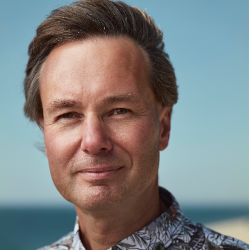
\includegraphics[width=.75\textwidth]{andy_stanford_clark1}
                \caption{\label{fig:andy}Andy Stanford-Clark da IBM}
            \end{figure}
        \end{column}
        \begin{column}{.5\textwidth}
            \begin{figure}[!htb]
                \centering
                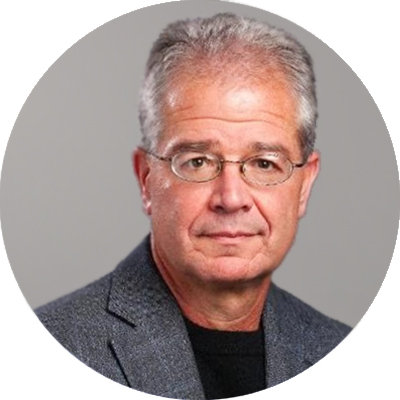
\includegraphics[width=.77\textwidth]{arlen_nipper1}
                \caption{\label{fig:arlen}Arlen Nipper da Cirrus Link/Eurotech}
            \end{figure}
        \end{column}
    \end{columns}
\end{frame}

\begin{frame}
    \frametitle{Problemas a serem resolvidos}
    \begin{itemize}
        \item Resolver o problema de conexão de oleodutos via satélite.
        \item Limitações:
            \begin{itemize}
                \item Alta latência;
                \item Baixa largura de banda;
                \item Dispositivos com pouca bateria.
            \end{itemize}
    \end{itemize}
        
\end{frame}

\begin{frame}
    \frametitle{Requisitos do Protocolo}
    \begin{itemize}
        \item Implementação simples;
        \item Uso de QoS, \textit{Quality of Service} por quem publica a mensagem;
        \item Uso eficiente de largura de banda, baixo \textit{overhead};
        \item Baixo custo energético para envio;
        \item Possibilidade de enviar qualquer tipo de dado;
        \item Possibilidade de manter conexões ativas, prontas para enviar e receber dados;
    \end{itemize}
\end{frame}

\begin{frame}
    \frametitle{Fase do protocolo proprietário}
    \begin{figure}[!htb]
        \centering
        
\includegraphics[width=\textwidth]{logo_mqtt}
        %\caption{\label{fig:logo_mqtt}Logo do MQTT}
    \end{figure}
    \begin{itemize}
        \item Primeira versão implementada no ano de 1999;
        \item Batizado MQTT, \textit{MQ Telemetry Transport}, em referência ao produto da IBM MQ Series
        \item Muito utilizado embarcado em produtos da IBM.
    \end{itemize}
\end{frame}

\begin{frame}[allowframebreaks]
    \frametitle{Fase do protocolo aberto}
    \begin{itemize}
        \item Demanda/Aplicabilidade IoT;
        \item Em 2010 o protocolo se tornou livre;
        \item Primeira versão lançada 3.1;
        \item Investimentos da IBM através da Eclipse Foundation para criar um ecossistema em torno do protocolo.
    \end{itemize}
    \begin{figure}[!htb]
        \centering
        
\includegraphics[width=.5\textwidth]{eclipse_logo}
        %\caption{\label{fig:eclipse_logo}Logo da Eclipse Foundation}
    \end{figure}
    \framebreak
    \begin{figure}[!htb]
        \begin{columns}[c]
            \begin{column}{.5\textwidth}
                
\includegraphics[width=.9\textwidth]{paho_logo}
            \end{column}
            \begin{column}{.5\textwidth}
                
\includegraphics[width=.9\textwidth]{Mosquitto_logo}
            \end{column}
        \end{columns}
        \caption{\label{fig:logos_ferramentas_mqtt}Exemplos de aplicações do ecossistema MQTT}
    \end{figure}
    \framebreak
    \begin{itemize}
        \item No ano de 2013 a IBM buscou padronização com a OASIS;
        \item 29 de outubro de 2014 o MQTT foi aprovado como padrão pela OASIS na sua versão 3.1.1
    \end{itemize}
    \begin{figure}[!htb]
        \centering
        
\includegraphics[width=.8\textwidth]{Oasis_logo}
        %\caption{\label{fig:Oasis_logo}}
    \end{figure}
\end{frame}

\begin{frame}
    \frametitle{Fase atual do protocolo}
    \begin{itemize}
        \item A última versão 5.0 março de 2019;
        \item Funcionalidades modernas como:
            \begin{itemize}
                \item facilidade de conexão e interação com a nuvem;
                \item Tratamento de erros;
            \end{itemize}
        \item Implementações de clientes para diversos sistemas e linguagens;
        \item Implementação de diversos brokers;
        \item Utilizado por grandes empresas tanto software aberto quanto proprietário.
    \end{itemize}
\end{frame}

\section{Aplicações}\label{Aplicacoes}

\begin{frame}
    \frametitle{Aplicações em IoT}
    \begin{itemize}
        \item Uso Doméstico e Educacional
        \item Uso Industrial
            \begin{itemize}
                \item BMW Mobility Services
                \item Matternet Autonomous Drones
            \end{itemize}
    \end{itemize}
    \begin{figure}
        \centering
        
\includegraphics[width=.4\textwidth]{drivenow_logo}
        
\includegraphics[width=.4\textwidth]{matternet_logo}
    \end{figure}
\end{frame}

\begin{frame}
    \frametitle{BMW Mobility Services}
    \begin{itemize}
        \item Drive Now;
        \item Serviço de compartilhamento de veículos;
        \item Realização de tarefas de modo remoto;
        \item Presença em 12 cidades na Europa;
        \item Uso do protocolo MQTT;
    \end{itemize}
     \begin{figure}[!htb]
         \centering
        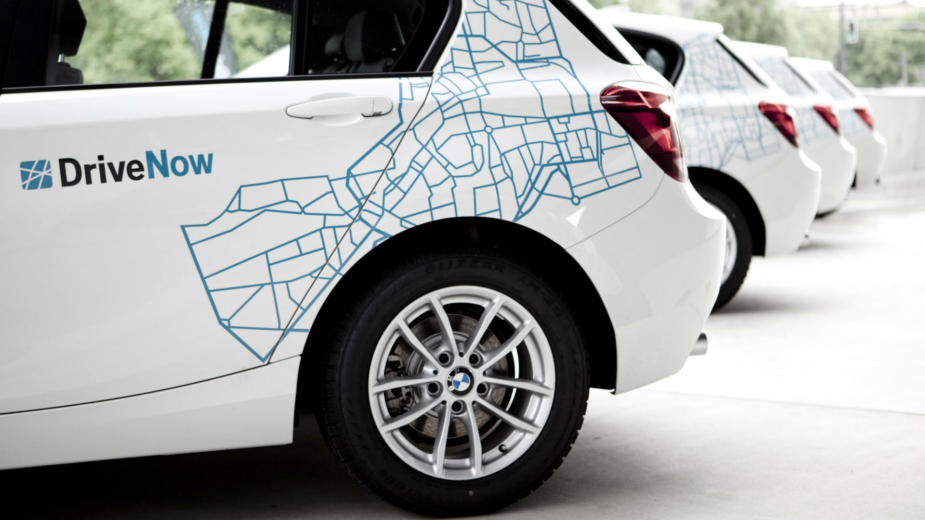
\includegraphics[width=.6\textwidth]{drive_now}
    \end{figure}
\end{frame}

\begin{frame}
    \frametitle{Matternet Autonomous Drones}
    \begin{itemize}
        \item Drones para transporte de amostras;
        \item Obrigatoriedades legais;
                \begin{itemize}
                    \item Monitoramento dos voos
                    \item Acesso em tempo real a dados
                    \item Controle remoto dos drones
                \end{itemize}
        \item Uso do protocolo MQTT;
    \end{itemize}
    \begin{figure}[!htb]
        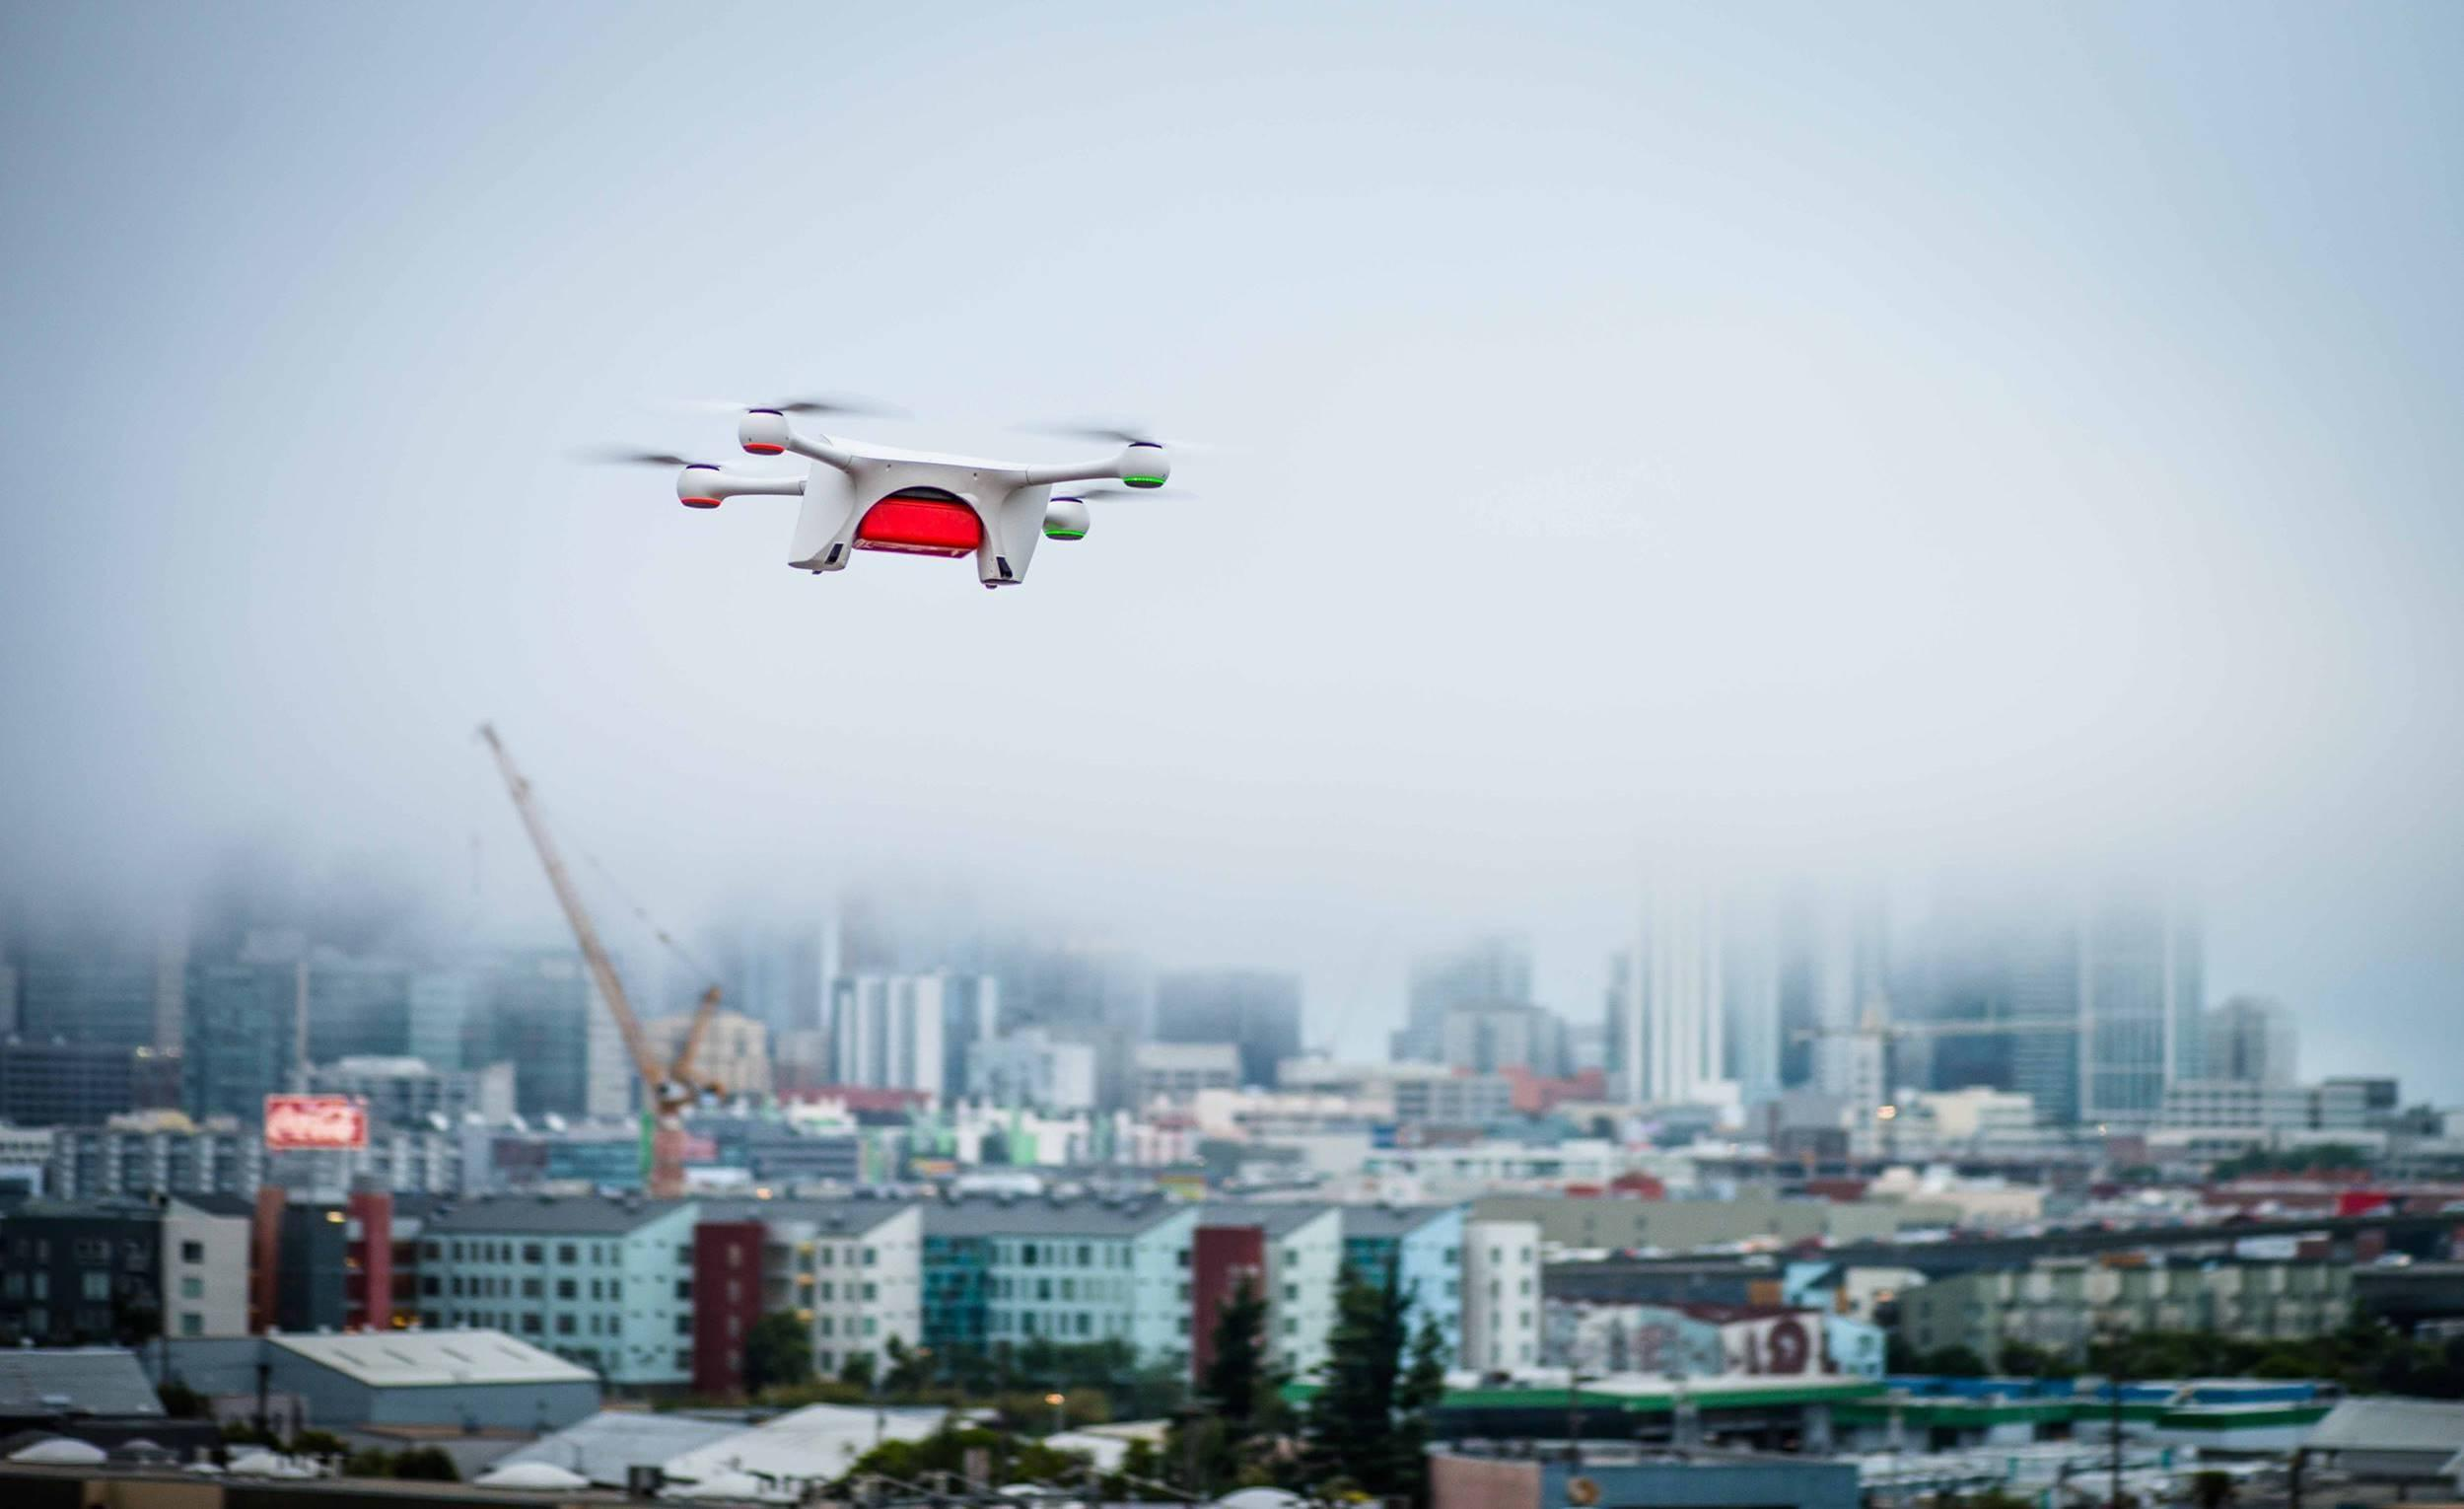
\includegraphics[width=.6\textwidth]{matternet_drone}
    \end{figure}
\end{frame}

\section{Embasamento teórico}\label{Embasamento teórico}

\begin{frame}[allowframebreaks]
    \frametitle{Embasamento teórico - Cliente}
    
    \textbf{Cliente}: programa ou dispositivo que irá enviar ou receber informação. Nesse sentido o cliente deve ser capaz de:
    \begin{itemize}
        \item iniciar uma conexão com o servidor,
        \item realizar a publicação de informações em tópicos,
        \item realizar a subscrição a tópicos de interesse,
        \item realizar o cancelamento de uma subscrição e,
        \item finalizar uma conexão com o servidor.
    \end{itemize}
    
\end{frame}

\begin{frame}[allowframebreaks]
    \frametitle{Embasamento teórico - Broker}
    
    \textbf{Broker}: programa ou serviço que intermediá e gerência a informação, o envio e recebimento de dados dos clientes, é comum se referir ao mesmo como servidor. Nesse sentido o servidor deve ser capaz de:
    \begin{itemize}
        \item gerencia as conexões como os clientes,
        \item gerenciar as mensagens publicadas pelos clientes,
        \item gerenciar as subscrições dos clientes e,
        \item retransmitir as mensagens recebidas aos clientes.
    \end{itemize}
    
\end{frame}

\begin{frame}[allowframebreaks]
    \frametitle{Embasamento teórico}
    \begin{itemize}
    		\item \textbf{Conexão de rede}: se refere ao serviço provido pelo protocolo de comunicação na camada subjacente (TCP/IP) ao protocolo MQTT, e que permite o envio de informação entre os dispositivos.
    		\item \textbf{Mensagem}: representa a informação que se deseja transmitir e que portanto constitui o objetivo da comunicação. De forma geral, e pelas caraterísticas do protocolo, a mensagem deve ocupar o mínimo espaço possível - na maioria dos casos é um único valor.
    		\item \textbf{Sessão}: se corresponde com o período de interação entre um cliente e um servidos, durante o qual é mantido um grupo de informações que representam o estado da comunicação, podendo ser composto por mais de uma conexão.
    		\item \textbf{Subscrição}: é o ato de que o cliente desempenha para indicar ao servidor interesse em receber atualizações sobre a mudança de um tópico. Dessa forma, uma subscrição se encontra composta por um Filtro de Tópicos, para um ou mais tópicos, e um valor indicando a Qualidade de Serviço deseja (QoS).
    		\item \textbf{Subscrição compartilhadas}: são subscrições que se encontram associadas com mais de uma sessão de comunicação entre o cliente e o servidor. Dessa forma, permitem um maior rango de padrões de comunicação.
    		\item \textbf{Caracteres mágicos}: também chamados de Wildcards, permitem ao cliente indicar interesse em receber notificações de mais um tópico, para isso fazendo uso de caracteres que definem o padrão dos tópicos desejados.
    		\item \textbf{Nome de Tópico}: rótulo ou identificador de uma informação específica dentro do broker e que é constantemente atualizada pelos cliente quando publicam uma nova informação no tópico.
    		\item \textbf{Filtro de Tópico}: é uma expressão contida numa subscrição é que se corresponde com um ou mais tópicos
    		\item \textbf{Paquete MQTT}: conjunto de informação útil à comunicação cliente-servidor envida através da conexão de rede. O protocolo MQTT especifica 15 tipos de pacotes diferentes, os quais serão especificados a continuação.
    \end{itemize}
    
\end{frame}

\section{Características técnicas}\label{Características técnicas}

\begin{frame}
    \frametitle{Estrutura básica dos pacotes}

    \begin{table}[h!]\caption{Estrutura básica comum a todos os pacotes MQTT.}
        \centering
        \begin{tabular}{|l|}
            \hline
            \textbf{Cabeçalho fixo}     \\ \hline
            \textbf{Cabeçalho variável} \\ \hline
            \textbf{Carga útil}         \\ \hline
        \end{tabular}
    \end{table}
    
\end{frame}

\begin{frame}
    \frametitle{Estrutura do cabeçalho fixo}
    \begin{table}[h!]\caption{Estrutura do cabeçalho fixo utilizado no protocolo MQTT.}
        \centering
        \resizebox{\textwidth}{!}{%
            \begin{tabular}{|c|cccccccc|}
                \hline
                \textbf{Bit} &
                \multicolumn{1}{m{.08\textwidth}|}{\textbf{7}} &
                \multicolumn{1}{m{.08\textwidth}|}{\textbf{6}} &
                \multicolumn{1}{m{.08\textwidth}|}{\textbf{5}} &
                \multicolumn{1}{m{.08\textwidth}|}{\textbf{4}} &
                \multicolumn{1}{m{.08\textwidth}|}{\textbf{3}} &
                \multicolumn{1}{m{.08\textwidth}|}{\textbf{2}} &
                \multicolumn{1}{m{.08\textwidth}|}{\textbf{1}} &
                \multicolumn{1}{m{.08\textwidth}|}{\textbf{0}} \\ \hline
                %\textbf{0} \\ \hline
                \textbf{Byte 1} & \multicolumn{4}{c|}{\textbf{Tipo de pacote MQTT}} & \multicolumn{4}{c|}{\textbf{Sinais específicos do pacote}} \\ \hline
                \textbf{Byte 2} & \multicolumn{8}{c|}{\multirow{2}{*}{\textbf{Espaço restante}}}                                                 \\ \cline{1-1}
                \textbf{. . .}  & \multicolumn{8}{c|}{}                                                                                          \\ \hline
            \end{tabular}%
        }
    \end{table}
    
\textbf{Sinais específicos do pacote}: complementa a informação do tipo do pacote.

\textbf{Espaço restante}: informação útil e de controle dependentes de cada tipo de pacote.

\end{frame}

\begin{frame}
    \frametitle{Tipos de pacotes}
    \begin{table}[]\caption{Tipos de pacotes utilizados pelo protocolo MQTT -- Parte I.}
        \centering
        \resizebox{\textwidth}{!}{%
            \begin{tabular}{|l|l|l|l|}
                \hline
                \multicolumn{1}{|c|}{Tipo} & \multicolumn{1}{c|}{Código} & \multicolumn{1}{c|}{Remetente} & \multicolumn{1}{c|}{Descrição} \\ \hline
                Reserved    & 0  & -        & Reservado                                \\ \hline
                CONNECT     & 1  & Cliente  & Solicitação 				de conexão     \\ \hline
                CONNACK     & 2  & Servidor & Confirmação de conexão                   \\ \hline
                PUBLISH     & 3  & Ambos    & Publicar mensagem                        \\ \hline
                PUBACK      & 4  & Ambos    & Publicar confirmação (QoS 1)             \\ \hline
                PUBREC      & 5  & Ambos    & Publicar recebimento (QoS 2 – parte 1)   \\ \hline
                PUBREL      & 6  & Ambos    & Publicar lançamento (QoS 2 – parte 2)    \\ \hline
                PUBCOMP     & 7  & Ambos    & Publicar conclusão (QoS 2 – parte 3)     \\ \hline
            \end{tabular}
        }
    \end{table}
\end{frame}

\begin{frame}
    \frametitle{Tipos de pacotes}
    \begin{table}[]\caption{Tipos de pacotes utilizados pelo protocolo MQTT -- Parte II.}
        \centering
        \resizebox{\textwidth}{!}{%
            \begin{tabular}{|l|l|l|l|}
                \hline
                \multicolumn{1}{|c|}{Tipo} & \multicolumn{1}{c|}{Código} & \multicolumn{1}{c|}{Remetente} & \multicolumn{1}{c|}{Descrição} \\ \hline
                SUBSCRIBE   & 8  & Cliente  & Solicitação de inscrição                 \\ \hline
                SUBACK      & 9  & Servidor & Confirmação de inscrição                 \\ \hline
                UNSUBSCRIBE & 10 & Cliente  & Solicitação de cancelamento de inscrição \\ \hline
                UNSUBACK    & 11 & Servidor & Confirmação de cancelamento de inscrição \\ \hline
                PINGREQ     & 12 & Cliente  & Solicitação de PING                      \\ \hline
                PINGRESP    & 13 & Servidor & Resposta de PING                         \\ \hline
                DISCONNECT  & 14 & Ambos    & Notificação de desconexão                \\ \hline
                AUTH        & 15 & Ambos    & Troca de autenticação                    \\ \hline
            \end{tabular}
        }
    \end{table}
\end{frame}

\begin{frame}[allowframebreaks]
    \frametitle{Tipos de pacotes}
    \begin{itemize}
        \item \textbf{CONNECT - Requisição de Conexão}
    		\item \textbf{CONNACK - Reconhecimento de conexão}
    		\item \textbf{PUBLISH - Publicar mensagem}
    		\item \textbf{PUBACK - Reconhecimento de publicação}
    		\item \textbf{PUBREC - Recebimento de publicação}
    		\item \textbf{PUBREL - Liberação de publicação}
    		\item \textbf{PUBCOMP - Publicação completada}
    		\item \textbf{SUBSCRIBE - Requisição de subscrição}
    \end{itemize}
\end{frame}

\begin{frame}[allowframebreaks]
    \frametitle{Tipos de pacotes}
    \begin{itemize}
    		\item \textbf{SUBACK - Reconhecimento de subscrição}
    		\item \textbf{UNSUBSCRIBE - Requisição de cancelamento de subscrição}
    		\item \textbf{UNSUBACK - Reconhecimento de cancelamento de subscrição}
    		\item \textbf{PINGREQ - Requisição de PING}
    		\item \textbf{PINGRESP - Resposta a uma Requizição de PING}
    		\item \textbf{DISCONNECT - Requisição de desconexão}
    		\item \textbf{AUTH - Intercambio de autentificações}
    \end{itemize}
\end{frame}

\section{Segurança}\label{Segurança}

\begin{frame}
    \frametitle{Fatores de Risco}
    \begin{itemize}
        \item Grande quantidade de dispositivos IoT
        \item Baixo suporte para mecanismos de segurança convencionais
        \item Ataques DDoS
        \item Roubo de informações
        \item Obtenção do controle dos dispositivos
    \end{itemize}
        
\end{frame}

\begin{frame}
    \frametitle{Ataques DDoS - Distributed Denial of Service}
    \begin{itemize}
        \item Um dos tipos de ataques mais comuns
        \item Interrupção no tráfego de servidores, serviços ou rede por meio de grande fluxo de pacotes;
        \item Botnets;
                \begin{itemize}
                \item Dispositivos infectados por malware
            \end{itemize}
        \item Dificuldade na verificação contra botnets;
    \end{itemize}
\end{frame}

\begin{frame}
    \frametitle{Soluções para Diminuição dos Riscos}
    \begin{itemize}
        \item Realização de autenticação;
        \item Uso de algoritmos e protocolos de criptografia;
        \item Uso de VPN;
        \item Detecção de atividades suspeitas;
        \item Secure MQTT
                \begin{itemize}
                    \item TLS - Transport Layer Security
                    \item Utilização da porta 8833
                    \item Formato de uso cadastrado na IANA (Internet Assigned Numbers Authority)
                \end{itemize}
    \end{itemize}
\end{frame}


\section{Prática}\label{Prática}
\begin{frame}
    \frametitle{Dispositivos e softwares da parte prática}
    \begin{itemize}
        \item Esp32:
            \begin{itemize}
                \item Sensor Adafruit BMP-280;
                \item Led embutido no Esp32;
                \item C/C++ (Framework Arduino e ESP-IDF);
            \end{itemize}
        \item Raspberry:
            \begin{itemize}
                \item Docker executando o broker mosquitto;
                \item Cliente inscrito no tópico ``\#''
            \end{itemize}
    \end{itemize}
\end{frame}

\begin{frame}
    \frametitle{Diagrama da aplicação}
    \begin{figure}[!htb]
        \centering
        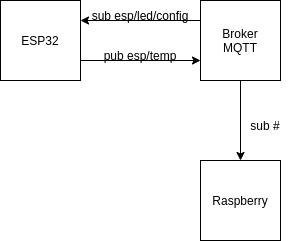
\includegraphics[width=.7\textwidth]{aplication}
        \caption{\label{fig:aplication} Dispositivos e tópicos utilizados}
    \end{figure}
\end{frame}

\begin{frame}[t,fragile,allowframebreaks]{\insertsectionhead}
    \frametitle{Códigos Fonte}
    \begin{lstlisting}
void setup() {
    if (!sensor.begin(BMP280_ADDRESS)) {
        if(!sensor.begin(BMP280_ADDRESS_ALT)) {
            delay(1000);
            ESP.restart();
        }
    }
    pinMode(LED_PIN, OUTPUT);
    wifiConnect();
    MqttConnect();
    xTaskCreate(taskSendTemperature, "send", 20000, NULL, 1, &handle);
}

void loop() {
    if (!mqttClient.connected()) {
        MqttConnect();
    }
    mqttClient.loop();
}
    \end{lstlisting}
\end{frame}

\begin{frame}
    \frametitle{Mão na massa!!}
    \begin{figure}
        \centering
        
\includegraphics[width=.3\textwidth]{pizza.png}
        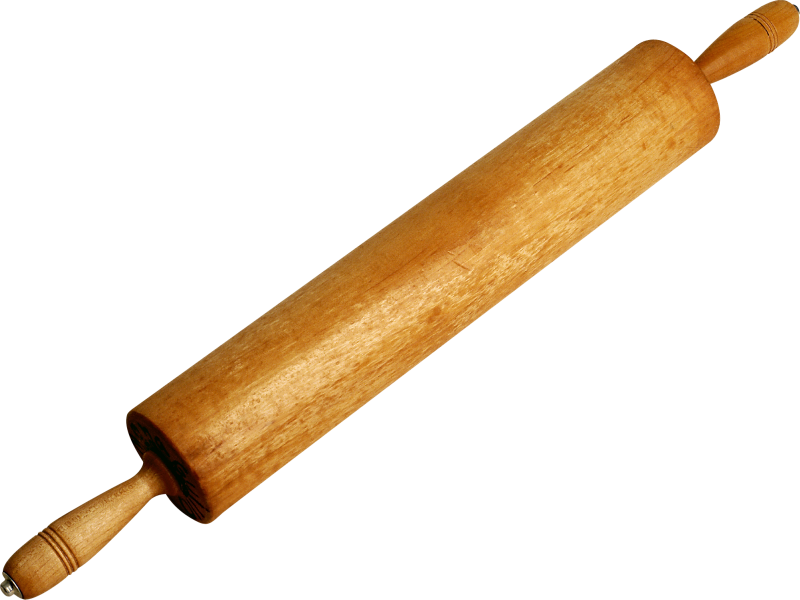
\includegraphics[width=.3\textwidth]{rolo.png}
        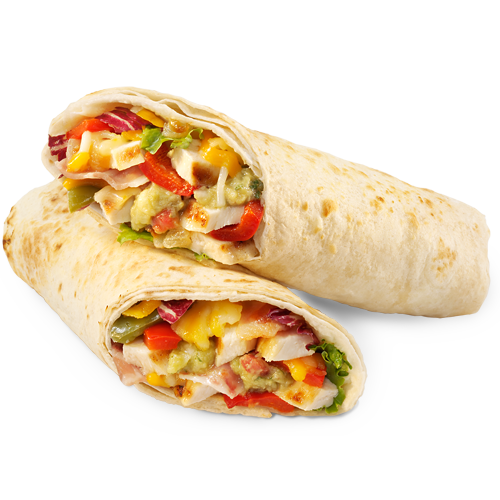
\includegraphics[width=.3\textwidth]{burrito.png}
    \end{figure}
\end{frame}

\section{Conclusão}
\begin{frame}
    \frametitle{Agradecimentos}
    \centering
    \Huge{Perguntas?}
    \begin{figure}
        \centering
        
\includegraphics[width=.3\textwidth]{alerta.png}
        
\includegraphics[width=.3\textwidth]{perigo.png}
        
\includegraphics[width=.3\textwidth]{eletricidade.png}
    \end{figure}
    \Huge{Obrigado pela atenção}
\end{frame}

\end{document}
